\documentclass{beamer}
%\documentclass[handout]{beamer}

\mode<presentation>
{
  %\usetheme{CambridgeUS}
  %\usetheme{Frankfurt}
  \usetheme{Singapore}
  %\usecolortheme{crane}
  \usefonttheme{professionalfonts}
  %\usefonttheme[onlymath]{serif}
  
  \setbeamertemplate{blocks}[rounded][shadow=true]
}

\usepackage{pgfpages}

\usepackage{alltt,verbatim,amsmath,times,empheq}
\usepackage{bm}
\usepackage[english]{babel}
\usepackage[utf8]{inputenc}

%\usepackage{times}
%\usepackage[T1]{fontenc}
% Or whatever. Note that the encoding and the font should match. If T1
% does not look nice, try deleting the line with the fontenc.

%\usepackage{hyperref}

\usepackage{pdfanim}
\usepackage{multimedia,xmpmulti}

\PDFAnimLoad[width=\textwidth,loop,interval=40]{exp3a}{exp3a/pic}{310}%

\usepackage{animate}

\definecolor{dark red}{HTML}{E41A1C}
\definecolor{dark green}{HTML}{4DAF4A}
\definecolor{dark violet}{HTML}{984EA3}
\definecolor{dark blue}{HTML}{084594}
\definecolor{dark orange}{HTML}{FF7F00}
\definecolor{light blue}{HTML}{377EB8}
\definecolor{light red}{HTML}{FB9A99}
\definecolor{light violet}{HTML}{CAB2D6}

\setbeamercolor{boxed}{fg=black,bg=uaf yellow}

\newcommand{\CC}{\mathbb{C}}
\newcommand{\NN}{\mathbb{N}}
\newcommand{\RR}{\mathbb{R}}
\newcommand{\ZZ}{\mathbb{Z}}
\newcommand{\Acal}{\mathcal{A}}
\newcommand{\Bcal}{\mathcal{B}}
\newcommand{\Ccal}{\mathcal{C}}
\newcommand{\Ncal}{\mathcal{N}}
\newcommand{\Kcal}{\mathcal{K}}

\newcommand{\bF}{\mathbf{F}}
\newcommand{\bQ}{\mathbf{Q}}
\newcommand{\bU}{\mathbf{U}}
\newcommand{\bbU}{\bar{\bU}}
\newcommand{\bu}{\mathbf{u}}
\newcommand{\bv}{\mathbf{v}}
\newcommand{\bx}{\mathbf{x}}

\newcommand{\Div}{\nabla\cdot}
\newcommand{\eps}{\epsilon}
\newcommand{\grad}{\nabla}
\newcommand{\lap}{\triangle}
\DeclareMathOperator{\trace}{tr}
\renewcommand{\bar}{\overline}

\newcommand{\ddx}[1]{\frac{\partial #1}{\partial x}}
\newcommand{\ddy}[1]{\frac{\partial #1}{\partial y}}
\newcommand{\pp}[2]{\frac{\partial #1}{\partial #2}}
\newcommand{\ppt}[1]{\frac{\partial #1}{\partial t}}
\newcommand{\ppT}[1]{\frac{\partial #1}{\partial T}}
\newcommand{\ppx}[1]{\frac{\partial #1}{\partial x}}
\newcommand{\ppy}[1]{\frac{\partial #1}{\partial y}}
\newcommand{\ppz}[1]{\frac{\partial #1}{\partial z}}
\newcommand{\ppxx}[1]{\frac{\partial^2 #1}{\partial x^2}}
\newcommand{\ppzz}[1]{\frac{\partial^2 #1}{\partial z^2}}

\newcommand{\Tnorm}[1]{\left|\!\left|\!\left|#1\right|\!\right|\!\right|}
\newcommand{\rhow}{\rho_{\text{w}}}
\newcommand{\Wq}{W^{1,q}(\Omega)}
\newcommand{\half}{\frac12}

%\setbeamercolor{redtext}{fg=red!80!black}
\setbeamercolor{redtext}{fg=red!94!black}
%\setbeamercolor{greentext}{fg=green!80!black}
\setbeamercolor{greentext}{fg=green!60!black}
%\setbeamercolor{bluetext}{fg=blue!70!black}
\setbeamercolor{bluetext}{fg=blue!90!black}
\setbeamercolor{yellowtext}{fg=yellow!95!black}
\setbeamercolor{orangetext}{fg=yellow!50!red}

\newcommand{\green}{\usebeamercolor[fg]{greentext}}
\newcommand{\blue}{\usebeamercolor[fg]{bluetext}}
\newcommand{\red}{\usebeamercolor[fg]{redtext}}

\renewcommand{\L}{\emph{Left}}
\newcommand{\R}{\emph{Right}}

\newcommand{\contactslipslide}{
\begin{frame}{sheets versus streams versus shelves}

\begin{columns}
\begin{column}{0.35\textwidth}
\small
\begin{itemize}
\small
\item non-sliding portions of ice sheets flow by shear deformation
\item ice streams slide: \alert{contact slip}
\item ``ice shelves'' are floating thick ice
\item ice shelves flow by extension
  \begin{itemize}
  \scriptsize
  \item[$\circ$] ``membrane'' or ``plug'' flow
  \end{itemize}
\end{itemize}
\end{column}

\begin{column}{0.65\textwidth}
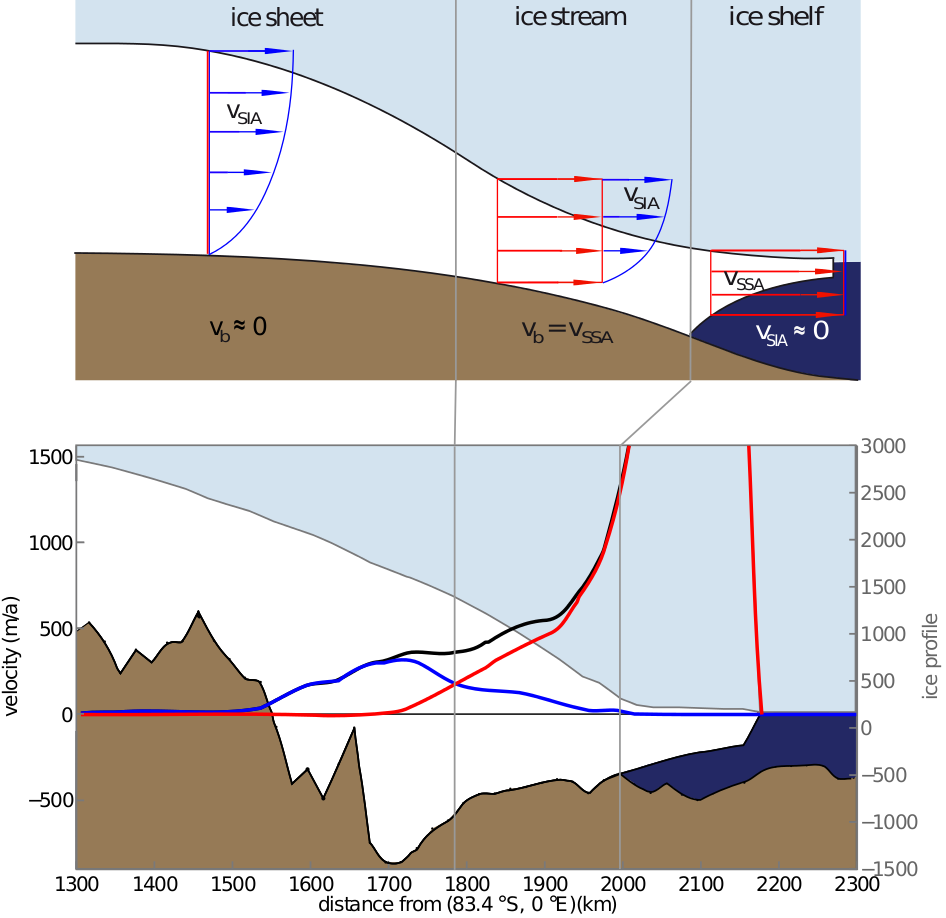
\includegraphics[width=1.1\textwidth]{siassacartoon-lambert}

\begin{center}
\vspace{-0.18in}
\tiny [Lambert glacier and Amery ice shelf, Antarctic]
\end{center}
\end{column}
\end{columns}
\end{frame}
}




\title[math and ice sheets]{An applied mathematician lives with \\ flowing ice sheets}

\author[Bueler]{Ed Bueler}

\institute[UAF]{
  \tiny Dept of Mathematics and Statistics and Geophysical Institute \\

  University of Alaska Fairbanks
}

\date{\tiny 21 May, 2014}


\setbeamerfont{date}{size=\scriptsize}

\subject{ice sheet modelling, ice sheets, ice streams, numerical analysis, applied mathematics}


%\begin{comment}
\AtBeginSection[]
{
  \begin{frame}<beamer>
    \frametitle{Outline}
    \tableofcontents[currentsection,hideallsubsections]
  \end{frame}
}
%\end{comment}


\begin{document}
%\graphicspath{{../commonfigs/},{/home/bueler/icerepo/UAF-misc/nwgm2012/figures/}}
\graphicspath{{../commonfigs/}}

\begin{frame}
  \titlepage
  \begin{center}
  \tiny supported by NASA grant NNX13AM16G
  \end{center}
\end{frame}



% NO OUTLINE BECAUSE ONE APPEARS AT START OF EACH SECTION ?
%\begin{comment}
\begin{frame}
  \frametitle{Outline}
  \tableofcontents[hideallsubsections]
  % You might wish to add the option [pausesections]
\end{frame}
%\end{comment}



\begin{frame}
  \frametitle{news from Antarctica}
  \framesubtitle{by Rignot et al.~(2014)}

\begin{center}

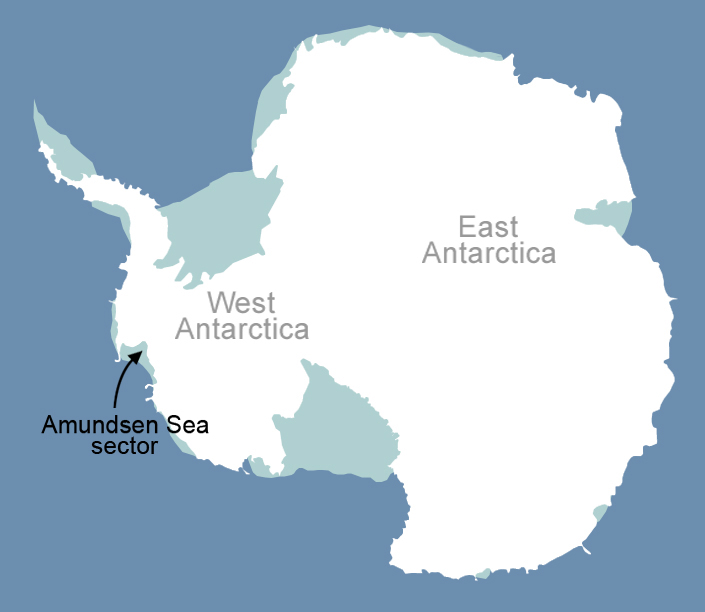
\includegraphics[width=0.55\textwidth]{antarctica-amundsen-sea-sector.png}

\bigskip
[show movie]
\end{center}
\end{frame}


\section[intro to ice sheet flow]{ice sheet flow: an introduction for non-glaciologists}



\begin{frame}{ice in glaciers is a viscous fluid}
\begin{columns}
\begin{column}{0.65\textwidth}
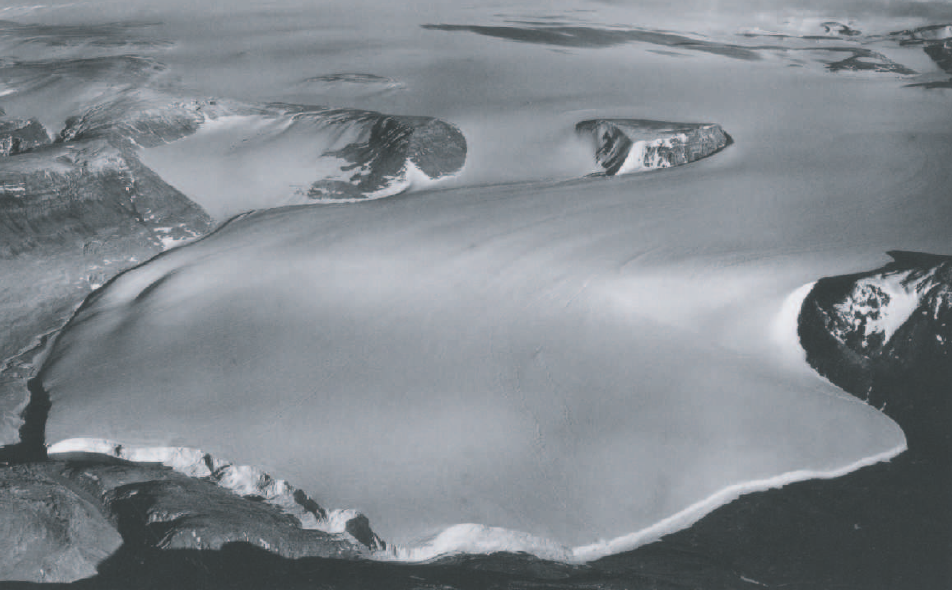
\includegraphics[width=1.0\textwidth]{polaris}
\end{column}
\begin{column}{0.35\textwidth}
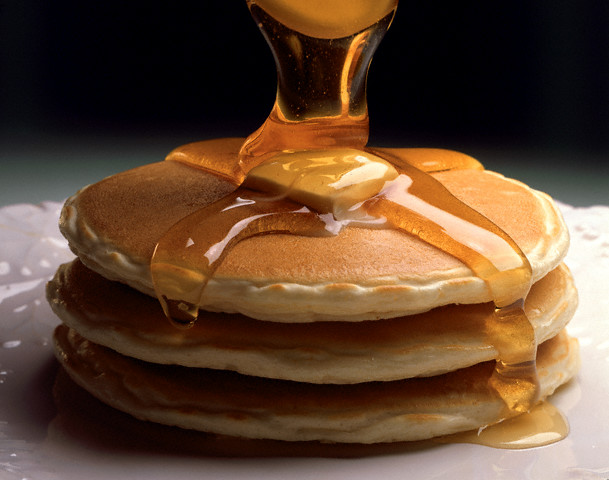
\includegraphics[width=1.0\textwidth]{pancakes}
\end{column}
\end{columns}

\bigskip\bigskip
\begin{itemize}
\item \dots at least: glaciers are viscous flows at larger scales
\item \emph{usage}: ``ice sheets'' are big, shallow glaciers
\end{itemize}
\end{frame}


\begin{frame}{ice in glaciers is a viscous fluid}

\begin{itemize}
\item primary variables: velocity $\mathbf{u}(\bx,t)$ and pressure $p(\bx,t)$
\item also: $\rho$ is density, $\mathbf{g}$ is gravity, $\nu$ is viscosity
\item if the glacier fluid were ``typical'' like the ocean we would model with Navier-Stokes equations:
\begin{align*}
\nabla \cdot \mathbf{u} &= 0 &&\text{\emph{incompressibility}} \\
\rho \left(\mathbf{u}_t + \mathbf{u}\cdot\nabla \mathbf{u}\right) &= -\nabla p + \nu \nabla^2 \mathbf{u} + \rho \mathbf{g} &&\text{\emph{stress balance}}
\end{align*}
\item but ice is not typical!
\item e.g.~not addressed in ice sheet flow models:
  \begin{itemize}
  \item[$\circ$] turbulence
  \item[$\circ$] convection
  \item[$\circ$] coriolis force
  \item[$\circ$] density-driven flow
  \end{itemize}
\end{itemize}
\end{frame}


\begin{frame}{ice is a slow, shear-thinning viscous fluid}

\begin{itemize}
\item our glacier fluid is
  \begin{enumerate}
  \item ``slow''\footnote{$Fr\approx 10^{-15}$.  Regarding coriolis: $Fr/Ro \approx 10^{-8}$.}:
    $$\rho \left(\mathbf{u}_t + \mathbf{u}\cdot\nabla \mathbf{u}\right) \approx 0 \qquad \iff \qquad \begin{pmatrix} \text{forces of inertia} \\ \text{are negligible} \end{pmatrix}$$
  \item non-Newtonian (shear-thinning):
    $$\text{viscosity $\nu$ is not constant}$$
  \end{enumerate}
\end{itemize}
\end{frame}


\begin{frame}{ice is a slow, shear-thinning viscous fluid}

\begin{itemize}
\item notation:
  \begin{itemize}
  \item[$\circ$] $\tau_{ij}$ is deviatoric stress tensor
  \item[$\circ$] $\mathbf{D}u_{ij}$ is strain rate tensor
  \end{itemize}
\smallskip
\item the standard ice flow model is Glen-law Stokes:
\begin{align*}
\nabla \cdot \mathbf{u} &= 0 &&\text{\emph{incompressibility}} \\
0 &= - \nabla p + \nabla \cdot \tau_{ij} + \rho \mathbf{g} &&\text{\emph{slow stress balance}} \\
\mathbf{D}u_{ij} &= A \left|\tau_{ij}\right|^{n-1} \tau_{ij} &&\text{\emph{Glen flow law}}
\end{align*}
\item $1.8 < n < 4.0$ ?  \quad \alert{when in doubt: $n=3$}
\medskip
\item $A>0$ is ``ice softness''
\end{itemize}
\end{frame}


\begin{comment}
\begin{frame}{because ice is a slow fluid \dots}

\begin{itemize}
\item  geometry, boundary stress, and viscosity determine velocity field and pressure instantaneously (i.e.~in the Stokes model)

\bigskip
\item \emph{thus}: a time-stepping ice sheet code recomputes the velocity field at every time step, without requiring previous velocity \footnote{to be a weatherman you've got to know which way the wind blows \dots but not to be a glaciologist}
\end{itemize}
\end{frame}
\end{comment}


\begin{frame}{ice sheets are shallow}

\vspace{-0.2in}
\small
\begin{itemize}
\item cross section of Greenland ice sheet at $71^\circ$ N
  \begin{itemize}
  \item[$\circ$] {\color{dark green}{green}} and {\color{dark blue}{blue}}: vertically-exaggerated version
  \item[$\circ$] in {\color{dark red}{red}}: without vertical exaggeration
  \end{itemize}
\end{itemize}
\normalsize

  \begin{center}
    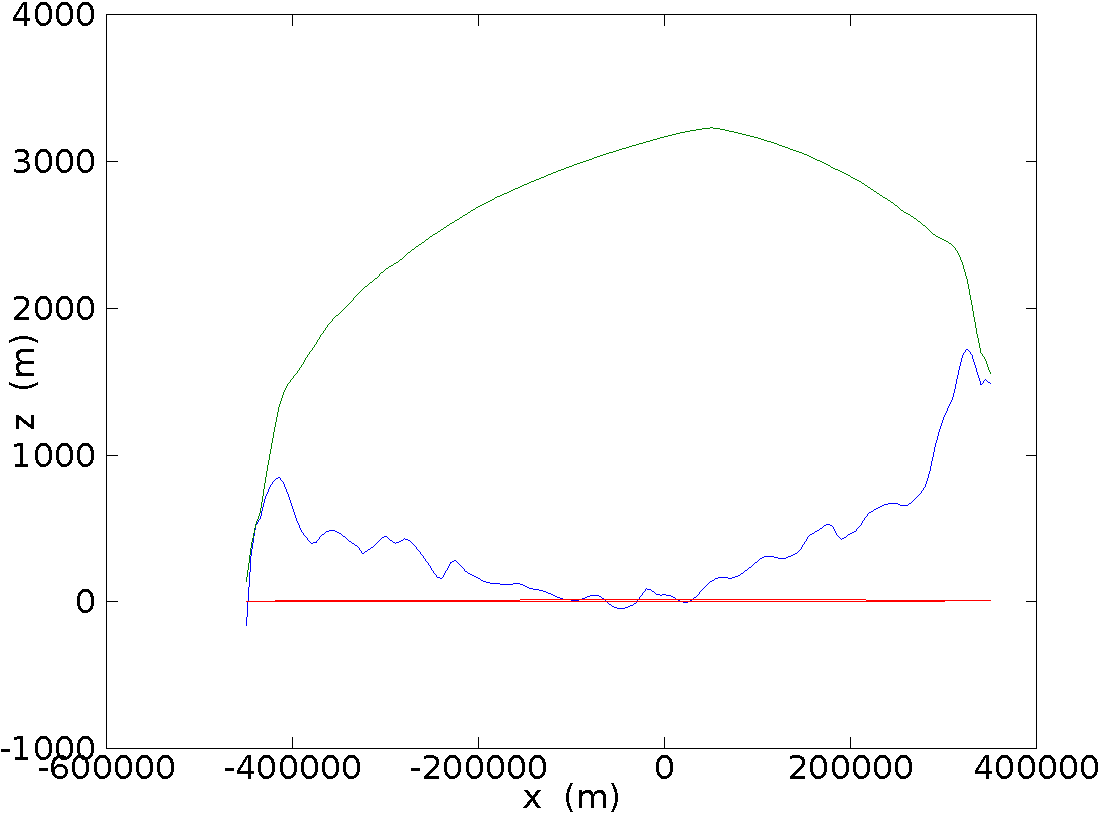
\includegraphics[width=0.7\textwidth]{greentrans}
  \end{center}
\end{frame}


\contactslipslide


\begin{frame}{outstanding viscous flows}

\begin{itemize}
\item ice sheets have four outstanding properties \emph{as viscous flows}:
  \begin{enumerate}
  \item \alert{slow}
  \item \alert{shear-thinning}
  \item \alert{shallow}
  \item \alert{contact slip}
  \end{enumerate}
\end{itemize}
\end{frame}


\begin{frame}
  \frametitle{big picture: ice sheet flow interacts with climate}

\medskip
\small
\begin{itemize}
\item \emph{mass and energy inputs}: (1) snow adds, (2) sun heats, (3) ocean heats, (4) earth heats
\item \emph{mass outputs}: (1) surface meltwater, (2) basal meltwater, (3) ice discharge
\end{itemize}

\begin{center}
  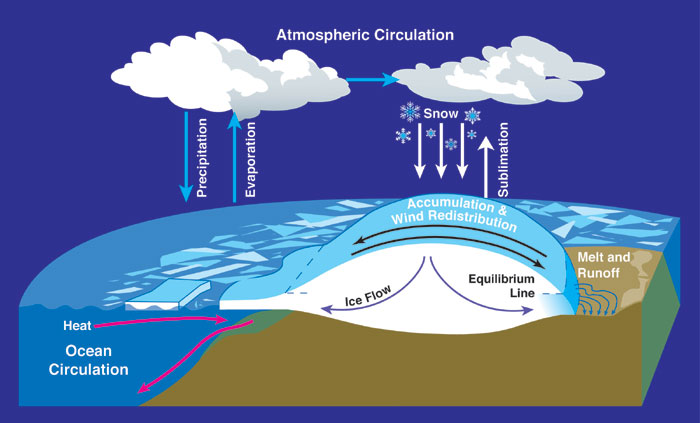
\includegraphics[width=0.75\textwidth]{mass-bal-atmos}
\end{center}
\end{frame}


\begin{frame}
  \frametitle{big picture: ice sheet changes over time}

\small
\begin{itemize}
\item ice sheet mass can be measured from space (!)
\item below: curves are ice sheet model $+$ climate model results
\item  Greenland ice sheet mass is $2.7 \times 10^9$ Gt \quad $(\approx \text{km}^3)$ % = 2.93466 10^6 km^3  volume, from SeaRISE-Greenland 5km data
\item  if \emph{all} Greenland ice melts: 7 m of sea level rise
\item  if \emph{all} Antarctic ice melts: 61 m of sea level rise
\end{itemize}
\normalsize

\begin{center}
    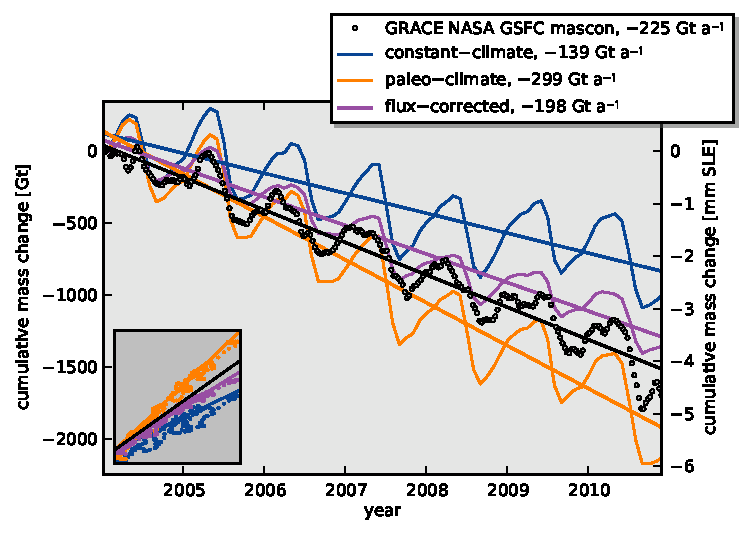
\includegraphics[width=0.7\textwidth]{ts_mass_2004-2010}
\end{center}
\end{frame}


\begin{frame}
  \frametitle{results from PISM}

\begin{itemize}
\item PISM = Parallel Ice Sheet Model (\texttt{pism-docs.org})
\item below are 2 km grid results for Greenland; everything evolves; only showing surface velocities
\end{itemize}

\vspace{-0.1in}
\begin{center}
    %\includegraphics<1>[height=4.2cm]{csurf_insar_pism_all} \\
    \includegraphics<1>[height=4.2cm]{speed_sar_pism_all} \\
   \footnotesize{a) observed; b) constant-climate; c) paleo-climate; d) flux-corrected}

\bigskip
\tiny (computations by Andy Aschwanden)
\end{center}
\end{frame}



\section[shallow ice approximation]{shallow ice approximation for grounded ice sheets}


\begin{frame}
  \frametitle{the main variables}

\begin{center}
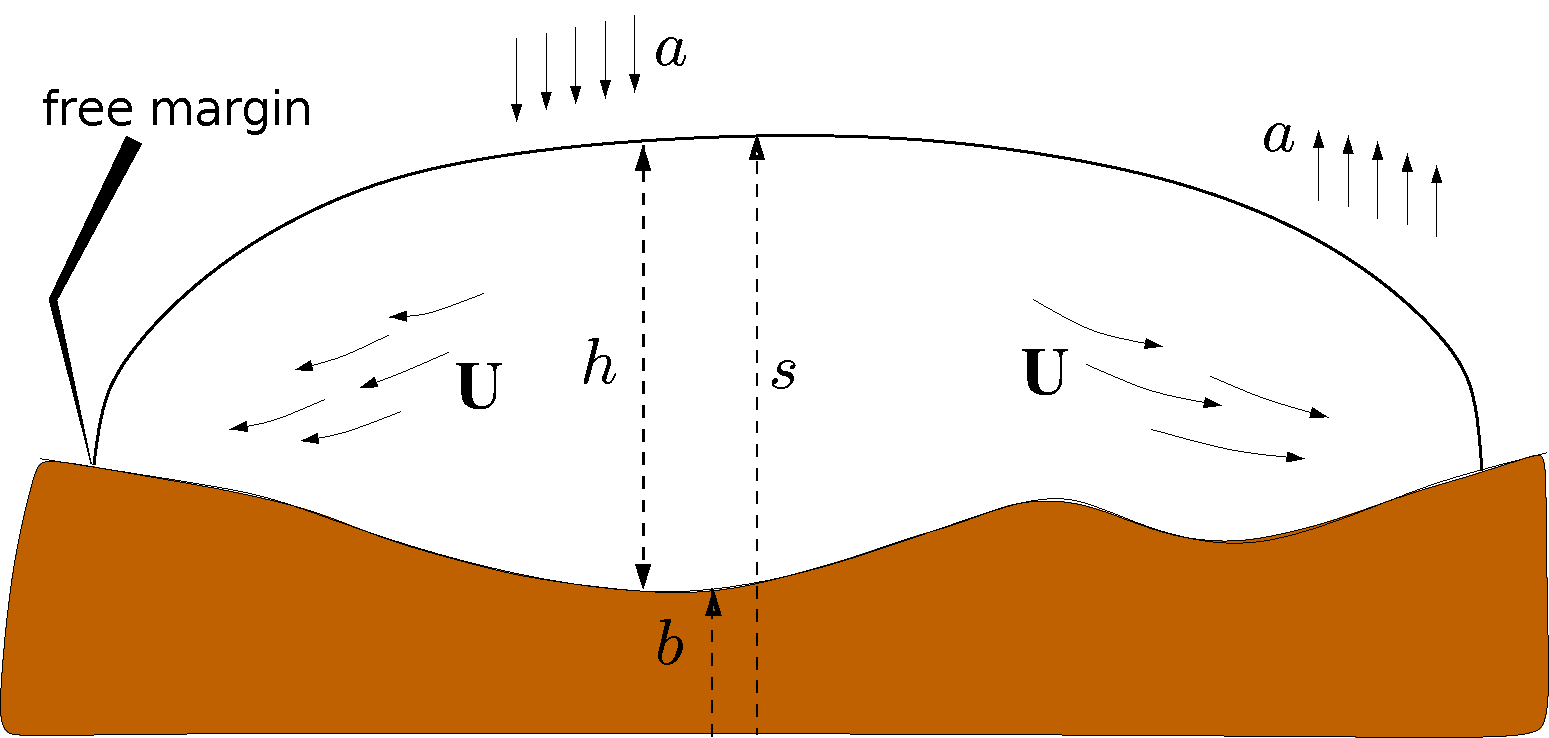
\includegraphics[width=0.7\textwidth]{groundedscheme}
\end{center}

\begin{itemize}
\small
\item $a(t,x,y,z)=$ yearly-average mass balance
\item $b(x,y)=$ bedrock elevation
\item $s(t,x,y)=$ ice surface elevation
\item $h(t,x,y)=$ ice thickness $ = s-b$
\item ${\bf U}(t,x,y,z)=$ horizontal velocity field
\end{itemize}

\begin{alertblock}{key idea: ice surface $s$ is always above the bedrock $b$}
\end{alertblock}
\end{frame}


\begin{frame}
  \frametitle{shallow ice approximation (SIA)}

\begin{itemize}
\item SIA = lubrication approximation of Stokes model
\item good approximation when:
  \begin{itemize}
  \item[$\circ$] sliding is small or zero
  \item[$\circ$] bedrock slope is modest
  \end{itemize}
\item derive SIA equations by scaling Stokes:
  \begin{itemize}
  \item[$\circ$] $[h]$ is a typical thickness scale
  \item[$\circ$] $[x]$ is a typical width scale
  \item[$\circ$] small parameter is $\eps = [h] / [x]$
  \end{itemize}
\end{itemize}
\end{frame}


\begin{frame}{movie of time-dependent SIA}

\begin{columns}
\begin{column}{0.4\textwidth}
\small
\begin{itemize}
\item at right is the Halfar similarity solution
\item an exact, time-dependent, zero mass balance solution where the $t\to 0^+$ limit is a delta function
\item compare Barenblatt solution of porous medium equation
\end{itemize}
\end{column}

\begin{column}{0.65\textwidth}
\vspace{-0.25in}

\begin{center}
\animategraphics[autoplay,loop,height=4.7cm]{4}{../commonfigs/animhalfar/halfar}{0}{26}

\bigskip
\tiny
frames from $t=4$ months to $t = 10^6$ years,

equal spaced in \emph{exponential} time
\end{center}
\end{column}
\end{columns}
\end{frame}


\begin{frame}
  \frametitle{SIA: velocity}
 
\begin{itemize}
\item let $p=n+1>2$
\item assume: no sliding and isothermal
\item horizontal ice velocity is given by: 
  $${\bf U}  =  - \frac{2 A}{p} (\rho g)^{p-1} \left[ (s-b)^p - (s - z)^p  \right] 
|\nabla s |^{p-2} \nabla s$$
\item no PDE needs to be solved to compute velocity!
\end{itemize}
\end{frame}


\begin{frame}
  \frametitle{SIA: steady state}

\begin{itemize}
\item mass conservation in steady state: 
  $$\Div \left(  \int_b^s {\bf U}\, dz \right)  =  a$$
\item shallow ice approximation + (steady) mass conservation:
  $$- \Div \left(\Gamma (s-b)^{p+1} | \nabla s |^{p-2} \nabla s  \right) =  a$$
  \begin{itemize}
  \vspace{-0.2in}
  \item[$\circ$] this is the major SIA equation (\dots a PDE?)
  \item[$\circ$] computes ice surface $s$
  \item[$\circ$] constant $\Gamma > 0$ combines $\rho,g,A,p$
  \item[$\circ$] $p$-Laplacish \dots but coefficient $(s-b)^{p+1} \to 0$ at margins
  \end{itemize}
\end{itemize}
\end{frame}






\begin{frame}
  \frametitle{SIA: an analogy}

\begin{columns}
\begin{column}{0.35\textwidth}
\begin{itemize}
\item ice sheet surface \\ = \alert{membrane}
\item bedrock = \alert{obstacle}
\end{itemize}
\vfill
\begin{center}
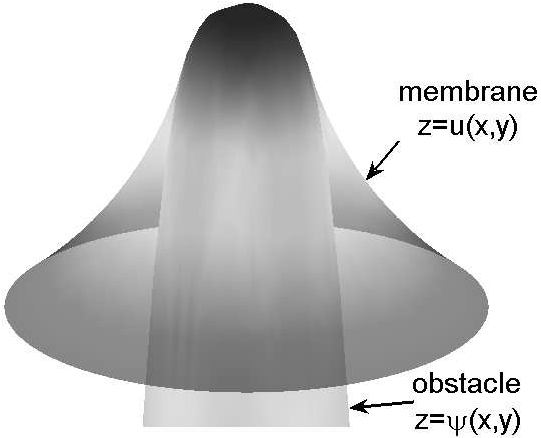
\includegraphics[width=1.1\textwidth]{classicalobs}
\end{center}
\end{column}
\begin{column}{0.65\textwidth}
\begin{center}
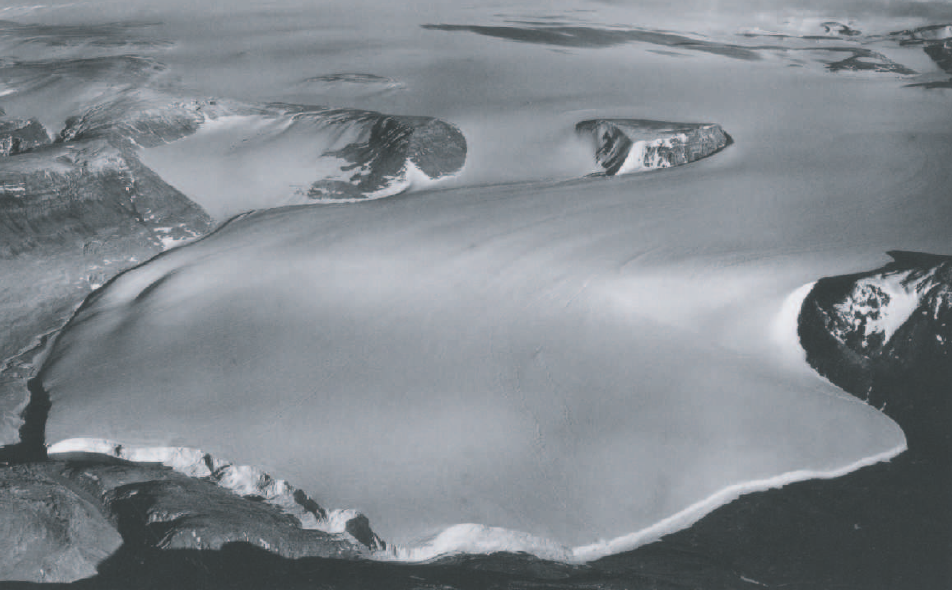
\includegraphics[width=0.8\textwidth]{polaris} \\
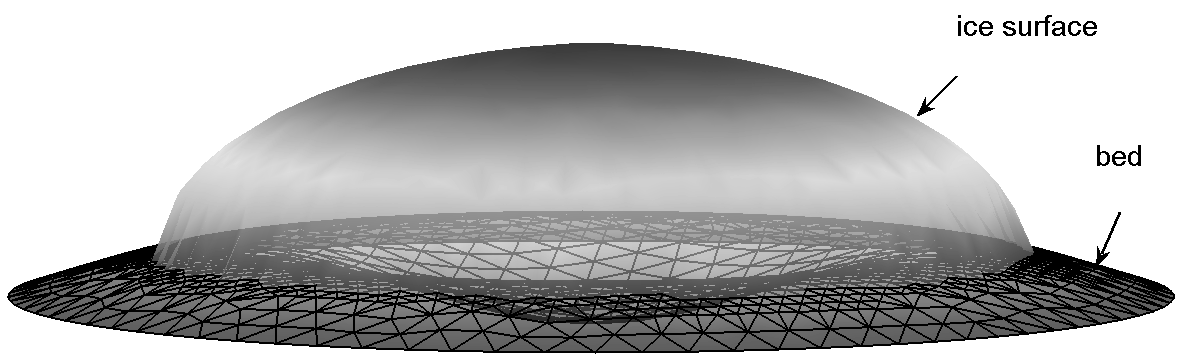
\includegraphics[width=\textwidth]{capnonflatobs}
\end{center}
\end{column}
\end{columns}
\end{frame}



\section{marine ice sheets}


\contactslipslide


\begin{frame}
  \frametitle{ice shelf versus sea ice}

\begin{center}
\vspace{-0.2in}

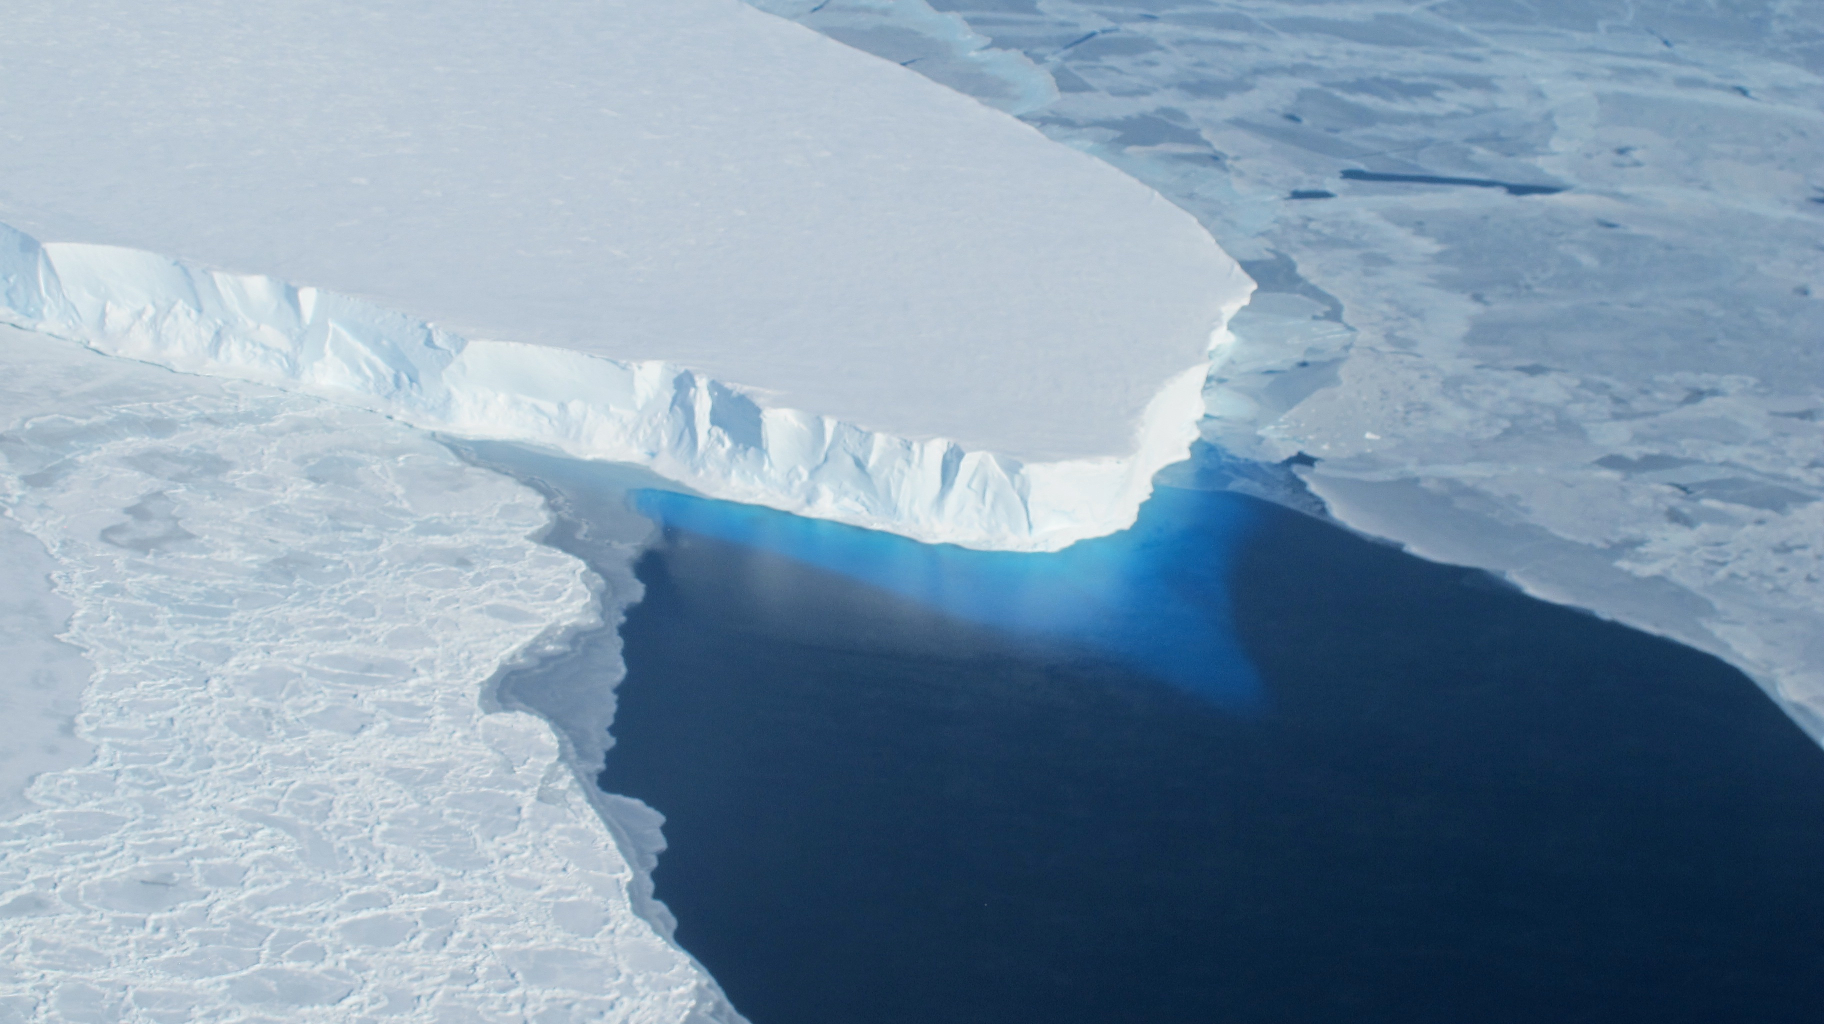
\includegraphics[width=1.0\textwidth]{supp4rignot-small}

\medskip
\tiny [ice shelf at Thwaites Glacier, Antarctic]
\end{center}
\end{frame}


\begin{frame}{models of ice shelves: they work}

\begin{itemize}
\item Ross ice shelf (Antarctica) velocity below
  \begin{itemize}
  \item[$\circ$] observed versus computed by SSA model in PISM
  \item[$\circ$] tuned: single, constant $A$
  \end{itemize}
\end{itemize}
\vspace{-0.3in}

\begin{center}
  \mbox{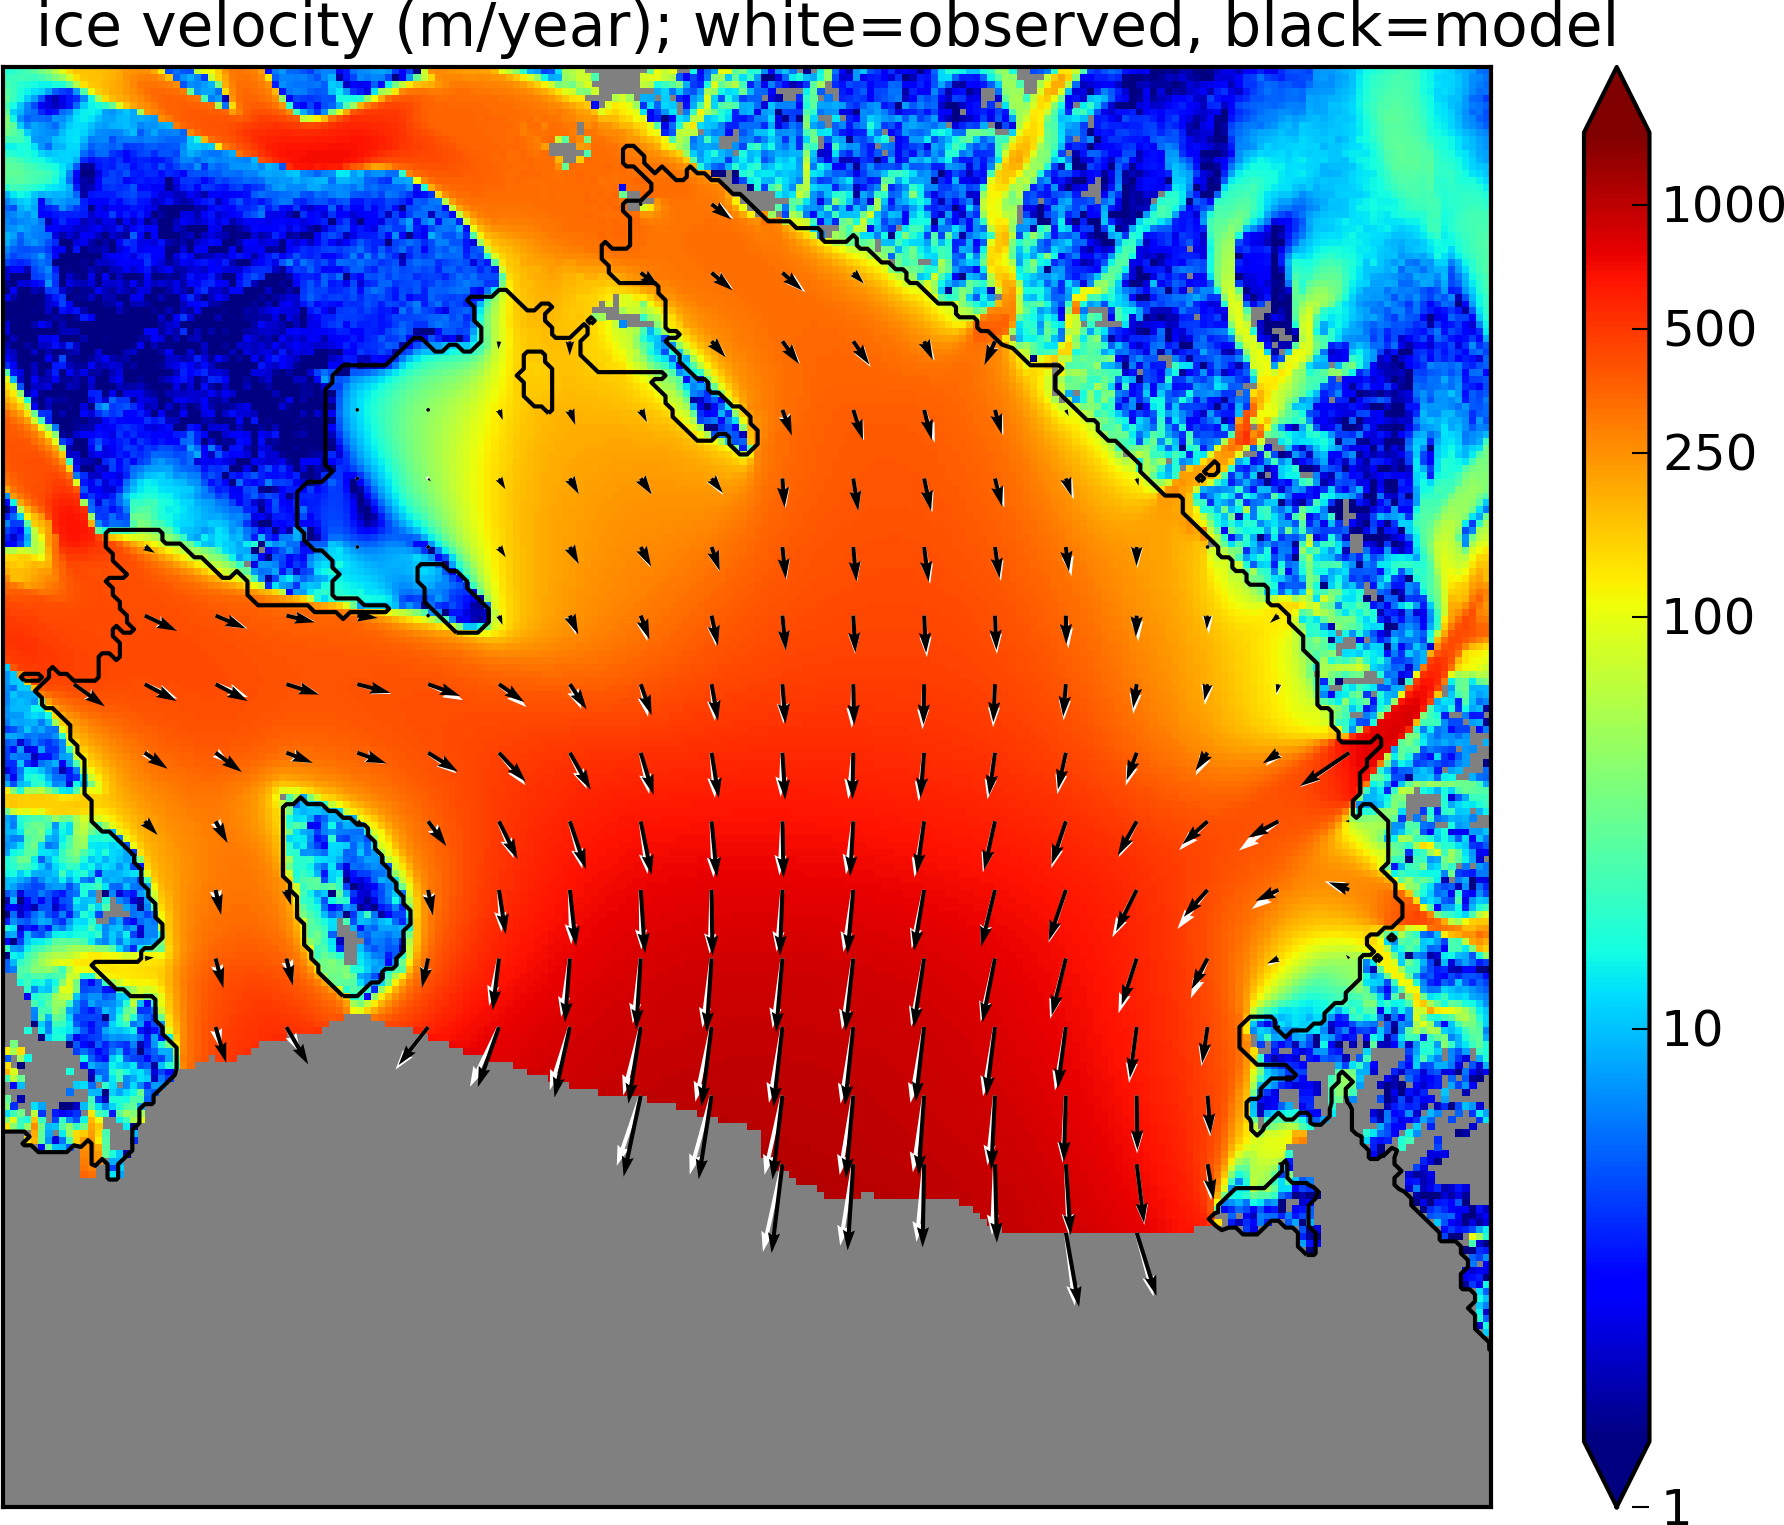
\includegraphics[width=0.58\textwidth]{rossquiver} \, 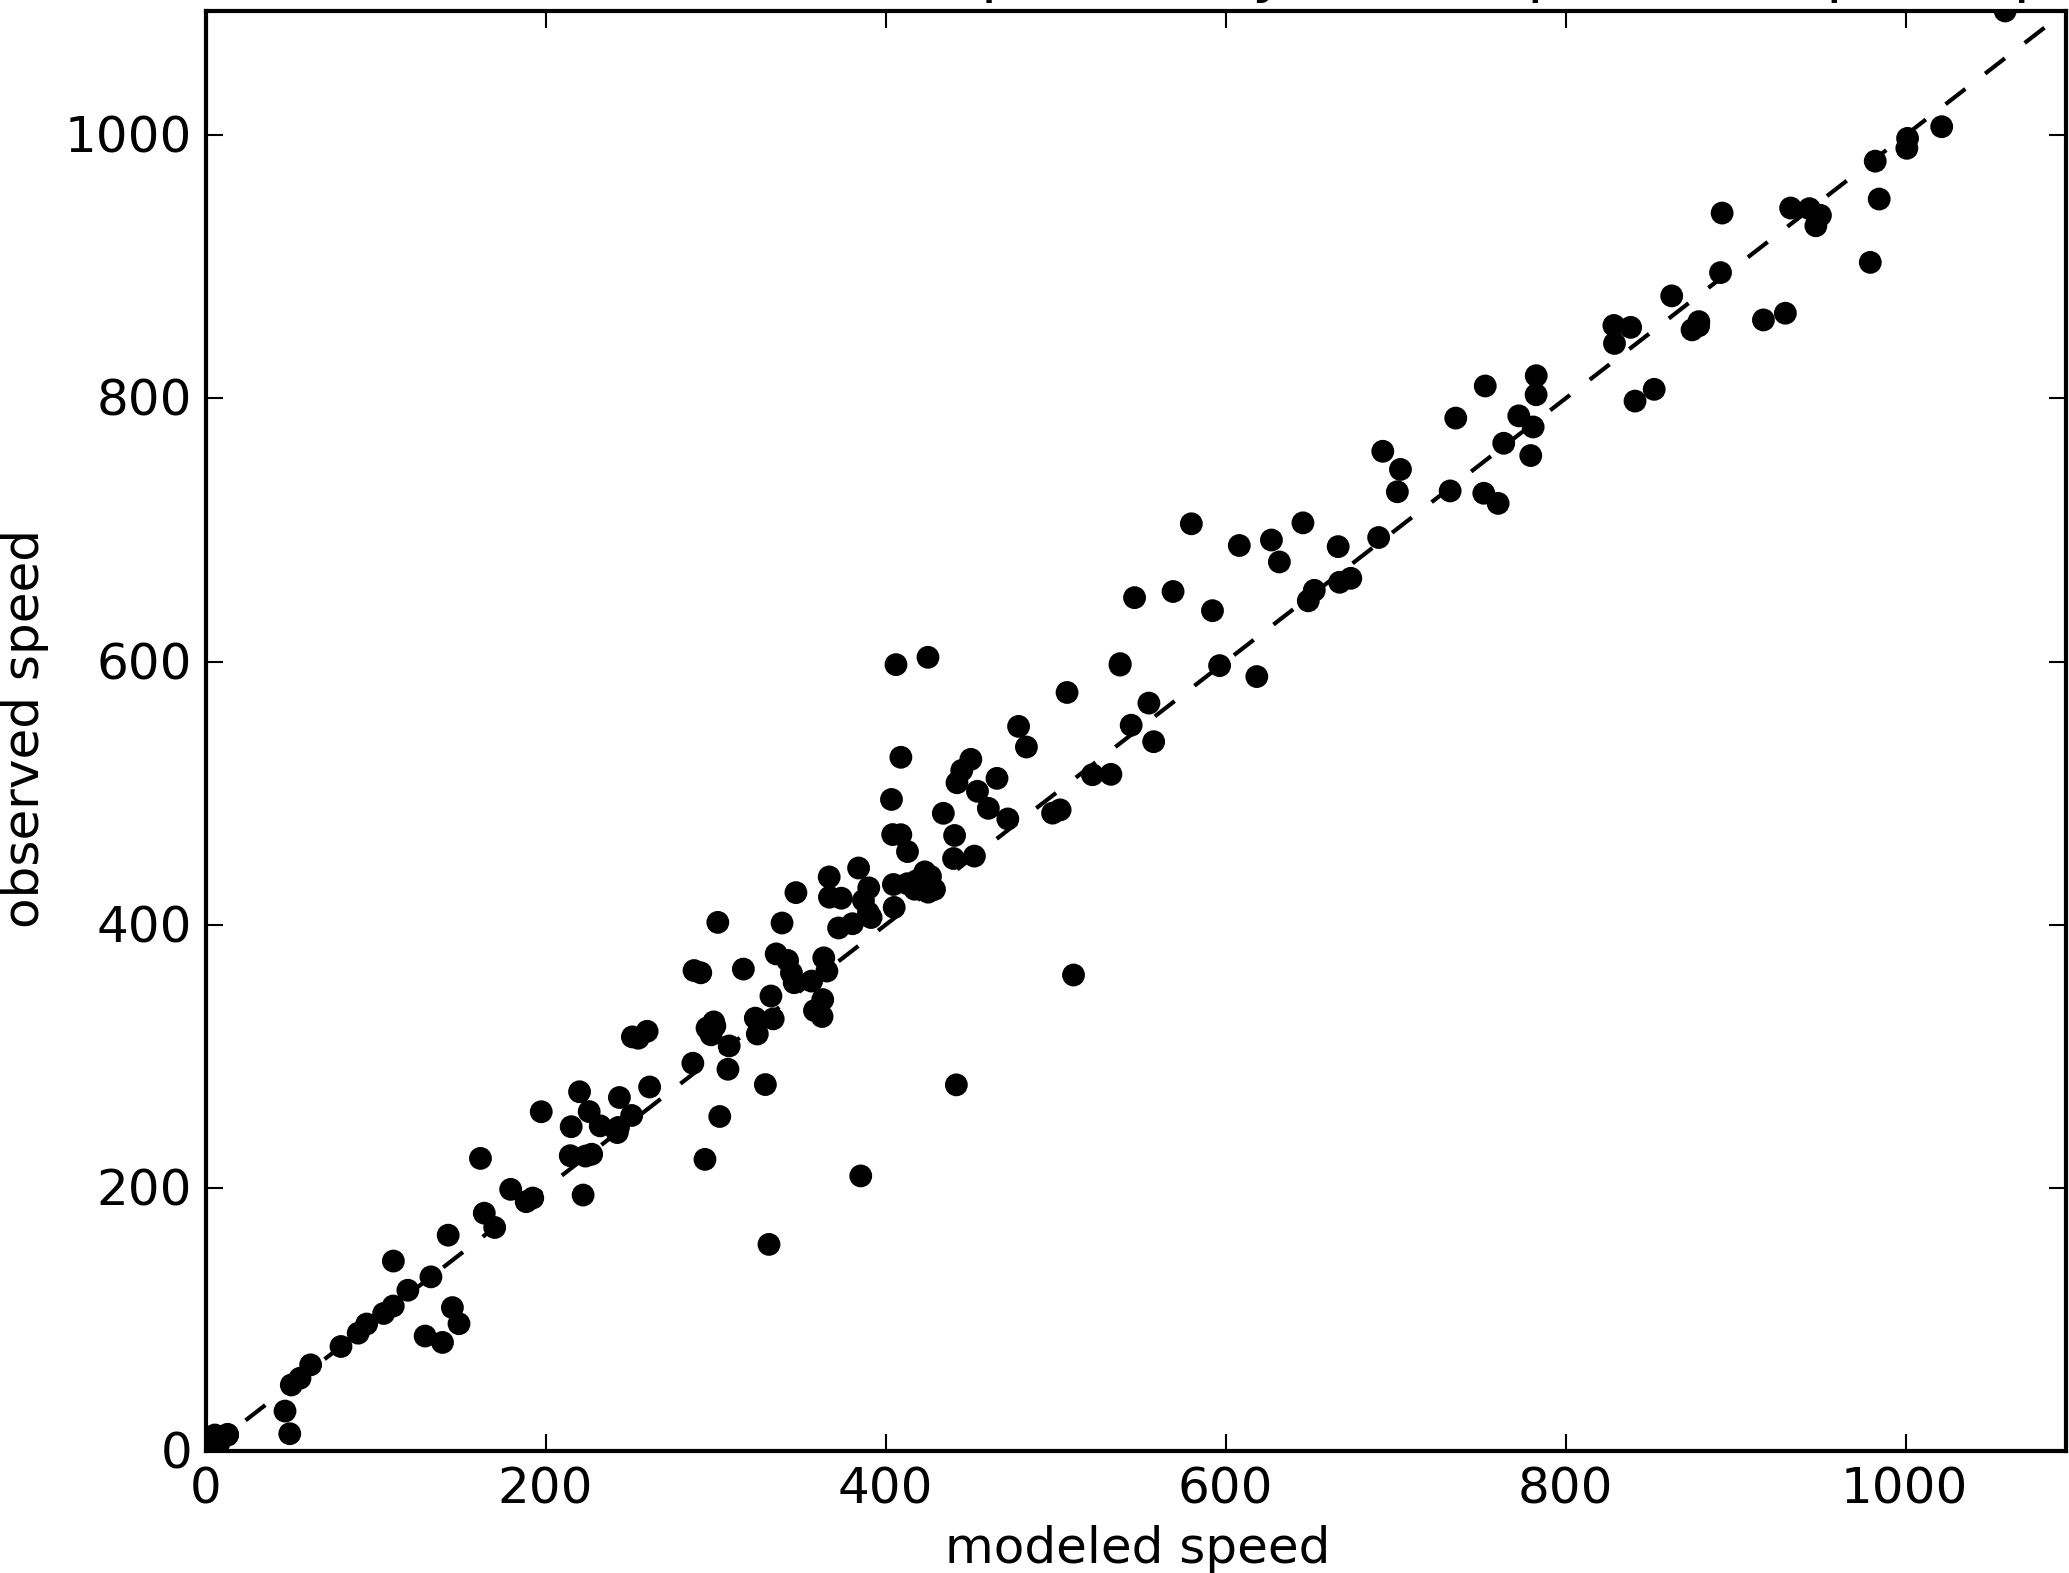
\includegraphics[width=0.48\textwidth]{rossscatter}}
\end{center}
\end{frame}


\begin{frame}
  \frametitle{ice streams: an analogy}

\begin{columns}
\begin{column}{0.6\textwidth}
\begin{itemize}
\item ice shelves have zero basal resistance
\item ice streams emerge where basal resistance is sufficiently low

(\emph{top}: Siple coast ice streams)
\item a basal resistance model:
  \begin{itemize}
  \item[$\circ$] ``plastic'' or Coulomb friction 
  \item[$\circ$] distribution of yield stress $\tau_c$
  \end{itemize}
\item ice membrane connects to upstream and/or lateral high friction with viscous stresses (\emph{bottom}: Schoof's slider analogy)
\end{itemize}
\end{column}
\begin{column}{0.4\textwidth}
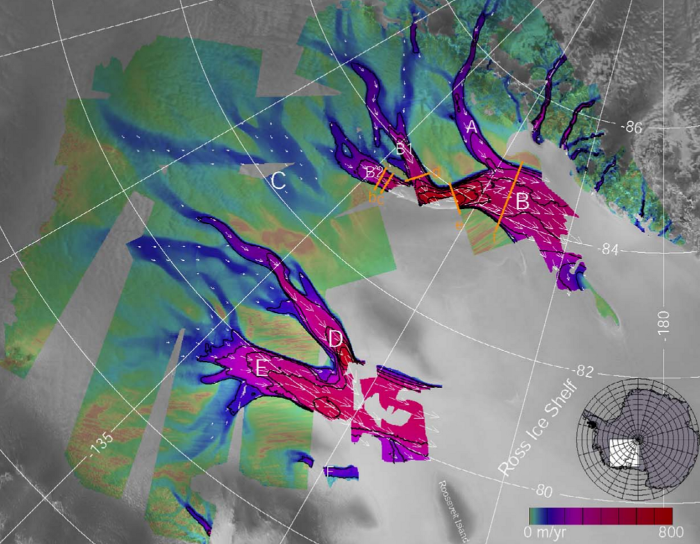
\includegraphics[width=\textwidth]{siple}

\vspace{0.3in}

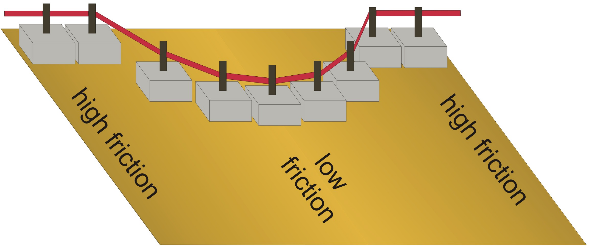
\includegraphics[width=1.1\textwidth]{schoof-sliders}
\end{column}
\end{columns}
\end{frame}


\begin{frame}
  \frametitle{moving grounding line in the lab}
  \framesubtitle{by Pegler et al.~(2014)}

\begin{center}

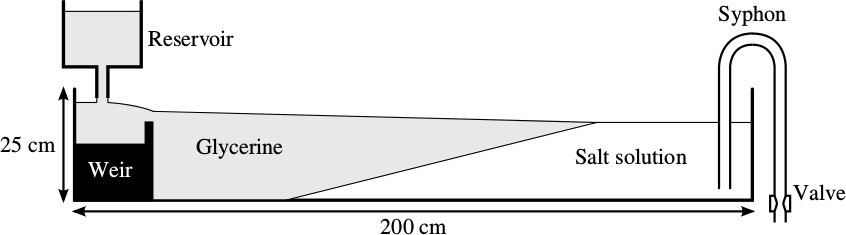
\includegraphics[width=0.7\textwidth]{pegler2014-grounding-line-schematic}

\vspace{1.0in}
[show movie]
\end{center}
\end{frame}


\begin{frame}
  \frametitle{a steady grounding line from the equations}
  \framesubtitle{by Bueler~(2014) submitted}

\begin{center}
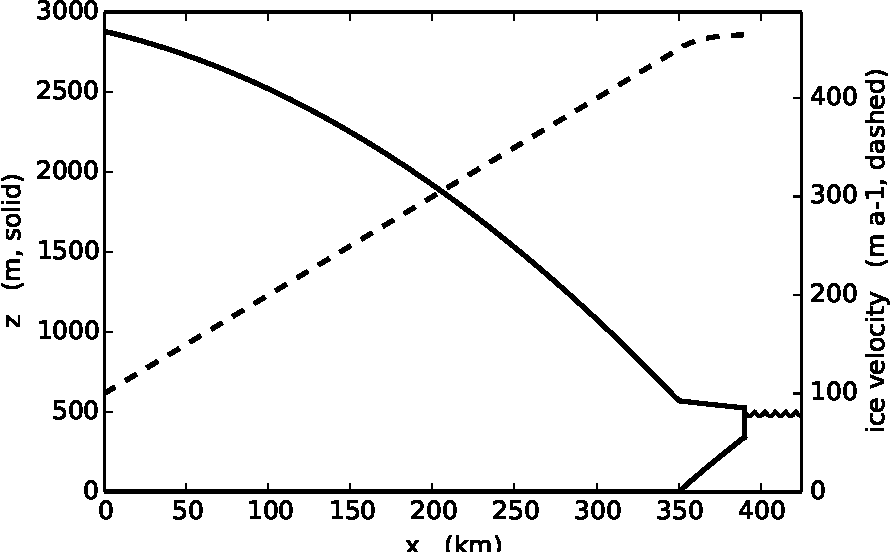
\includegraphics[width=0.8\textwidth]{exactmarine-geometry}
\end{center}

\vspace{-0.2in}

\small
\begin{itemize}
\item thickness (solid) and velocity (dashed) exactly solve the coupled equations for conservation of mass and momentum
\item \dots but I'll leave those equations unstated
\end{itemize}
\normalsize
\end{frame}







\section*{conclusion}

\begin{frame}
  \frametitle{conclusion}
  \framesubtitle{thanks for listening!}

\begin{center}
\animategraphics[autoplay,loop,height=6.5cm]{3}{anim/thwaitesframes}{0}{72}

\bigskip
\tiny
Thwaites glacier area, West Antarctica, from February 2002 to February 2014  (Rignot et al.~2014)
\end{center}

\end{frame}


\end{document}
